\section{Results}

\textit{São Félix do Xingu} has a growing trend of DETER warnings from August 
2016 to July 2021, where 2018 presents a particularly worrying peak. There are increases
in the warning areas of DETER along all sizes (see 
Figure~\ref{fig:deter_warnings_area_size}).

\begin{figure}[h] 
    \begin{center}
    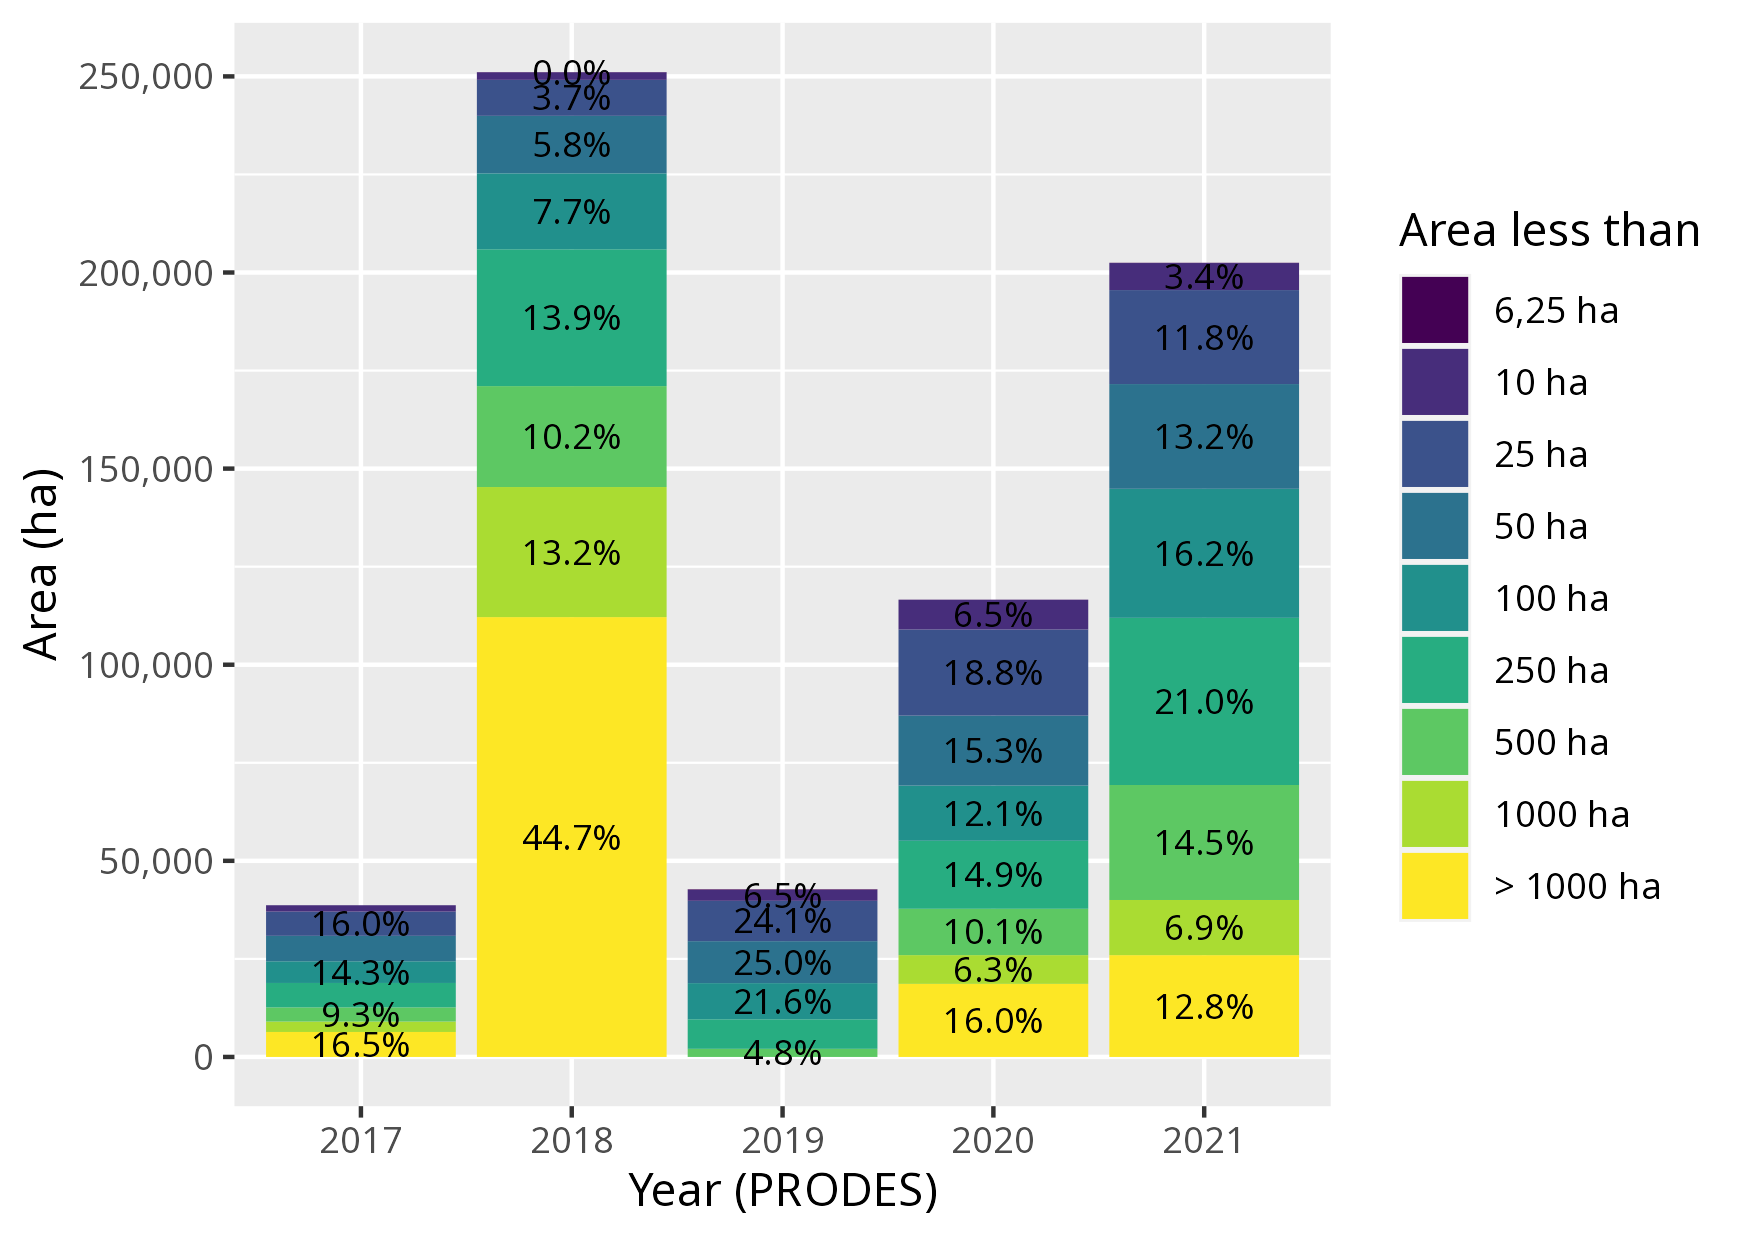
\includegraphics[width=\linewidth]{deter_warnings_area_size.png}
    \caption{Area of DETER warnings by year and size. The area covered by 
        warnings peaked in 2018. Note the increasing trend since 2019
        and how their distribution is homogeneous along the size brackets in 
        2021.}
    \label{fig:deter_warnings_area_size}
    \end{center}
\end{figure}

Meanwhile, the number of DETER warnings displays the same growing trend except
for the 2018 peak that isn't very prominent, indicating an increment not only 
in the number of DETER warnings, but also in their size (see 
Figure~\ref{fig:deter_warnings_size}).

\begin{figure}[h] 
    \begin{center}
    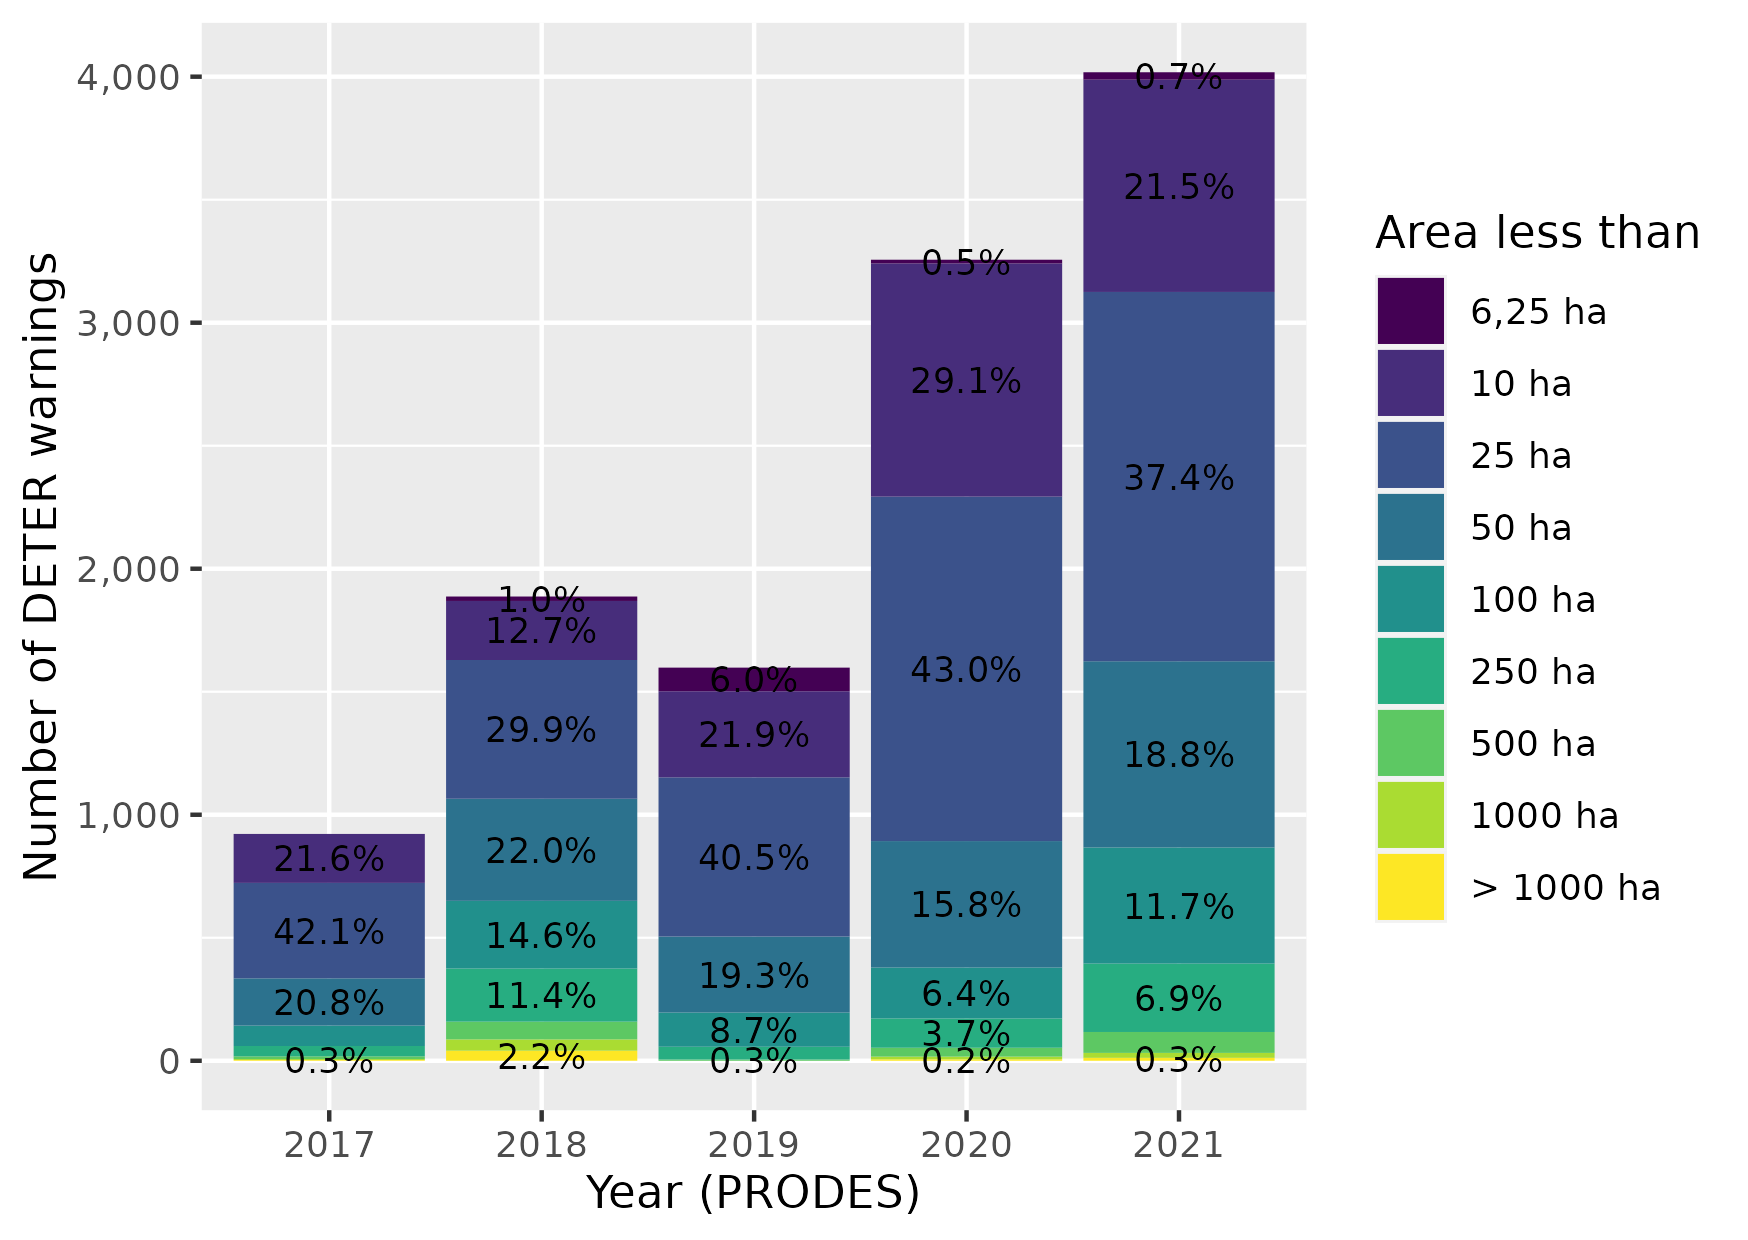
\includegraphics[width=\linewidth]{deter_warnings_size.png}
    \caption{Number of DETER warnings by year and size.Note the increasing 
        trend since 2017. The increase in warnings in 2018 corresponds to a
        large increase in area, implying an increment in the size of each 
        warning.}
    \label{fig:deter_warnings_size}
    \end{center}
\end{figure}

The month where most DETER warnings are issued in the area of interest during
the study period is September (the end of the 2-month dry season in half of the
Amazon~\cite{carvalho2021}), followed by October and August.
The yearly increasing trend is also found inside September and October (even 
the 2018 peak), the months with the most warnings, (see 
Figure~\ref{fig:deter_warnings_size_month}). 

\begin{figure}[h] 
    \begin{center}
    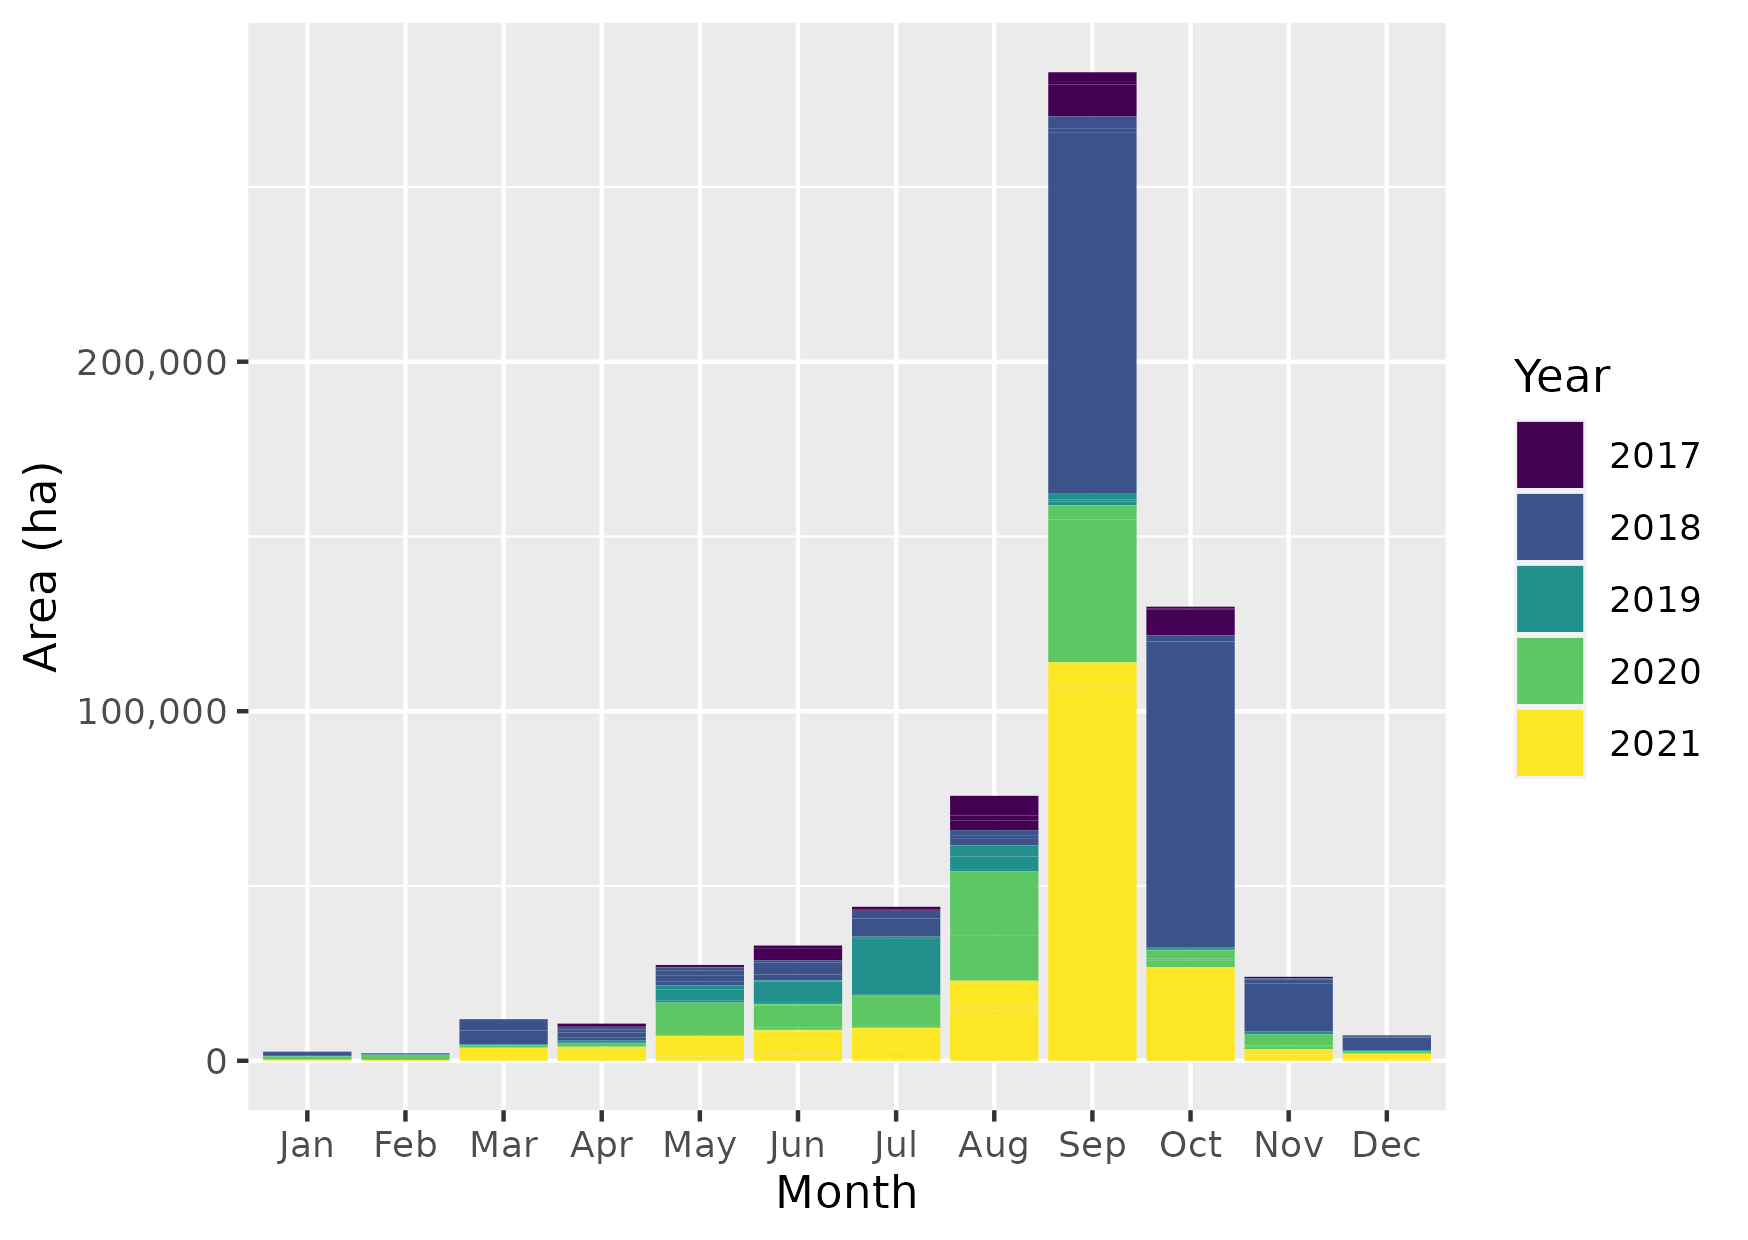
\includegraphics[width=\linewidth]{deter_warnings_size_month.png}
    \caption{DETER warnings by month. Between August and October is when most
        of the warnings are issued. Note how September presents an increasing 
        trend along the years on which 2018 is comparable to 2021.}
    \label{fig:deter_warnings_size_month}
    \end{center}
\end{figure}

Our analysis also shows that most subareas in the area of study receive only 
one DETER warning (see Figure~\ref{fig:plot_area_by_warnings}) and those which 
receive a second one, they receive it two or three years after (see 
Figure~\ref{fig:plot_days_first_to_last} and 
Table~\ref{tab:warnings_subareas_by_number_area}). 
% NOTE: Why aren't they receiving their second warnings one year after?
The remaining subareas, which receive a third or even a fourth waning, receive 
their last warning between three and four years after the first one (see 
Figure~\ref{fig:plot_days_first_to_last}).

\begin{figure}[h] 
    \begin{center}
    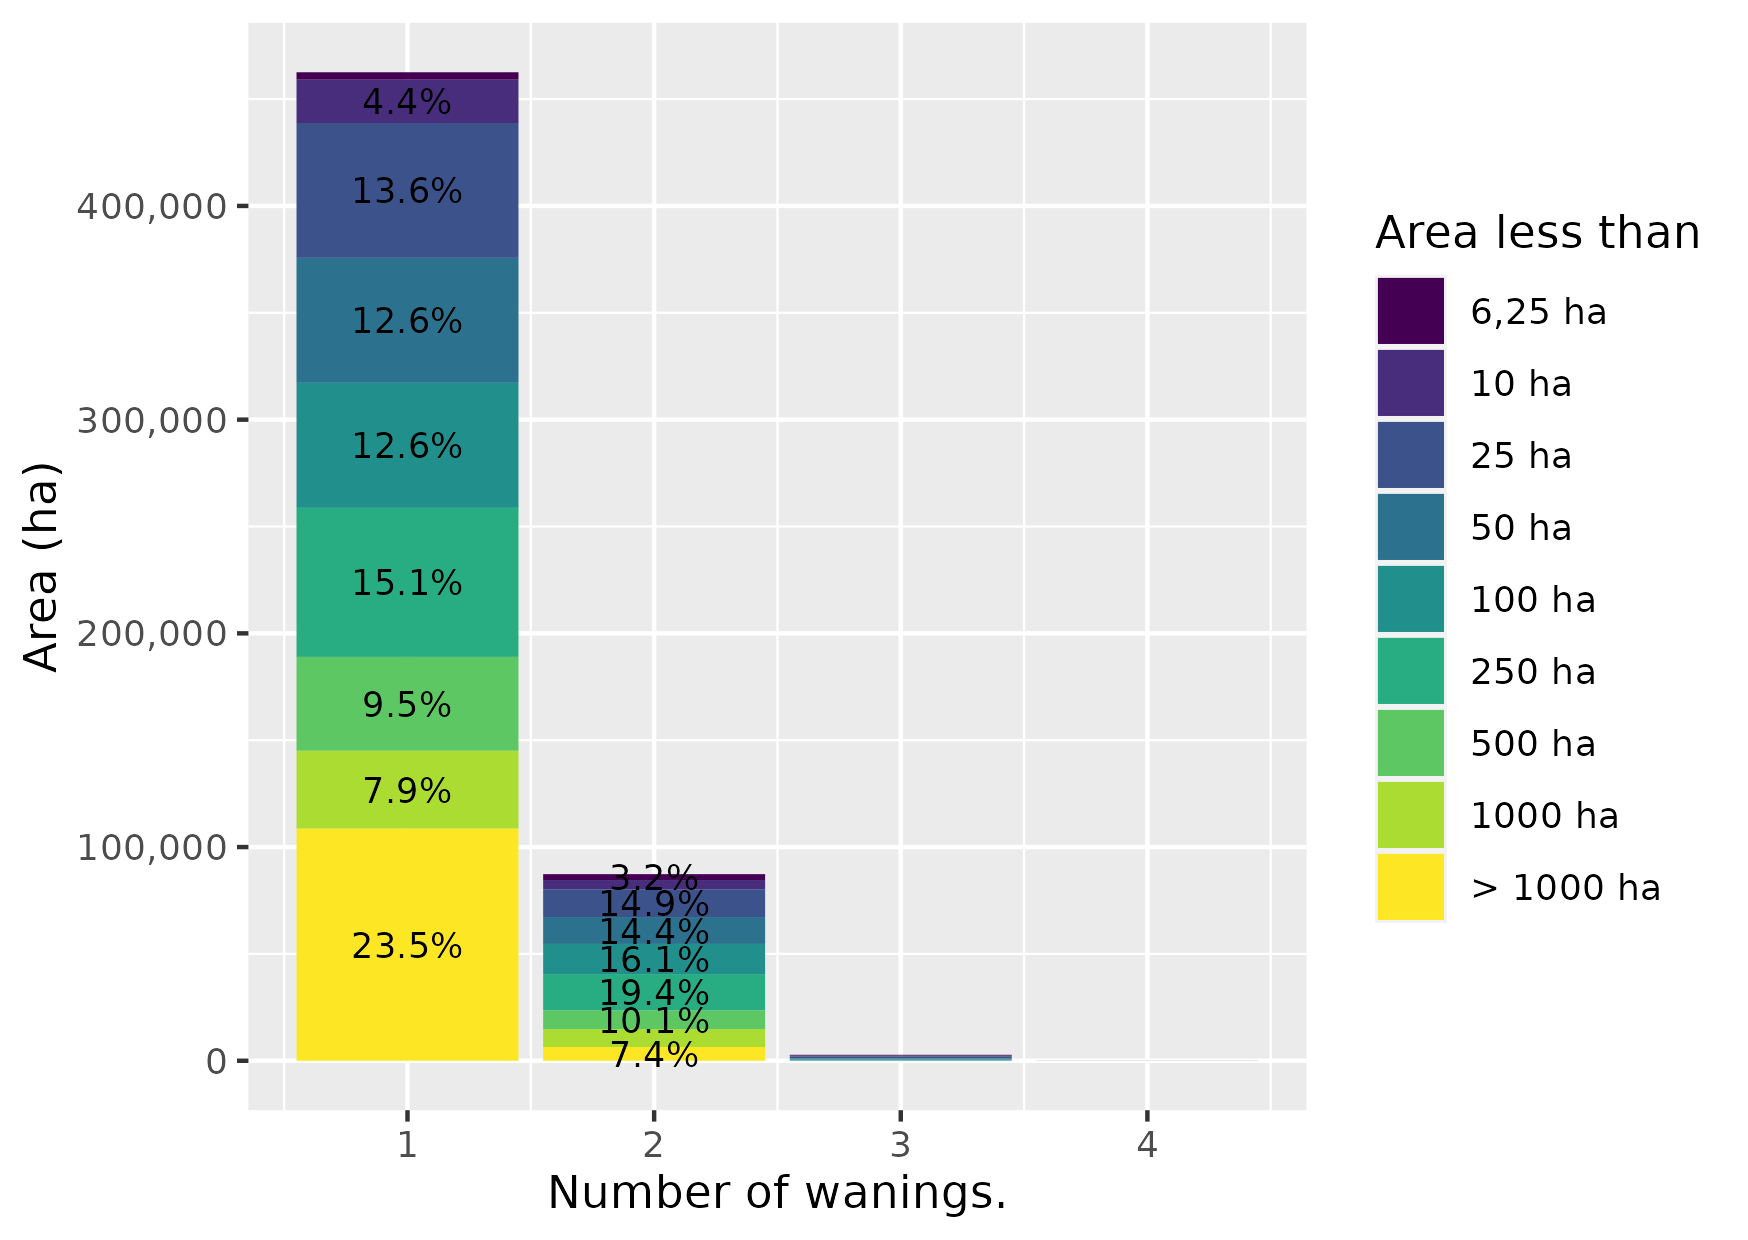
\includegraphics[width=\linewidth]{plot_area_by_warnings.png}
    \caption{DETER warning area by number of warnings. Most subareas are issued
        a DETER warning only once, and never more than four.}
    \label{fig:plot_area_by_warnings}
    \end{center}
\end{figure}

\begin{table}[h] % use [t] here to force table to top
    \centering
    \begin{tabular}{|c|c|r|r|}
        \hline
        \textbf{N. Warnings} & \textbf{Type} & 
        \textbf{N. Subareas} & \textbf{Total area}  \\
        \hline
1 & 6.25 ha    &  749  &   3468.9 \\ 
1 & 10 ha      & 2535  &  20277.6 \\
1 & 25 ha      & 4002  &  63098.2 \\
1 & 50 ha      & 1682  &  58496.4 \\
1 & 100 ha     &  847  &  58490.3 \\
1 & 250 ha     &  459  &  69741.0 \\
1 & 500 ha     &  133  &  43890.2 \\
1 & 1000 ha    &   54  &  36388.0 \\
1 & > 1000 ha &   42  & 108701.0  \\
        \hline
2 & 6.25 ha    &  617  &   2754.4 \\
2 & 10 ha      &  542  &   4300.3 \\
2 & 25 ha      &  829  &  13016.6 \\
2 & 50 ha      &  356  &  12588.7 \\
2 & 100 ha     &  200  &  14101.6 \\
2 & 250 ha     &  111  &  16949.5 \\
2 & 500 ha     &   25  &   8804.5 \\
2 & 1000 ha    &   12  &   8361.2 \\
2 & > 1000 ha &    3  &   6444.0  \\
        \hline
3 & 6.25 ha    &   70  &    331.8 \\
3 & 10 ha      &   48  &    383.2 \\
3 & 25 ha      &   62  &    943.4 \\
3 & 50 ha      &   15  &    528.5 \\
3 & 100 ha     &    5  &    342.0 \\
3 & 250 ha     &    2  &    261.5 \\
        \hline
4 & 6.25 ha    &    5  &     24.4 \\
4 & 10 ha      &    1  &      8.4 \\
4 & 25 ha      &    2  &     31.4 \\
        \hline
    \end{tabular}
    \caption{DETER warning subareas by number of wanings, type, number of 
    subareas, and total area. The number and total area decreases as the number
    of warnings increase.}
    \label{tab:warnings_subareas_by_number_area}
\end{table}


Besides, subareas smaller than 50 or 100 ha and two DETER warnings tend to 
receive their second waning two years after the first while larger subareas 
tend to receive them after three years (see the medians in 
Figure~\ref{fig:plot_days_first_to_last}). 
Something similar happens to subareas with 3 warnings, where subareas smaller 
than 25 ha receive their last warning approximately one year before than larger 
subareas.

\begin{figure}[h] 
    \begin{center}
    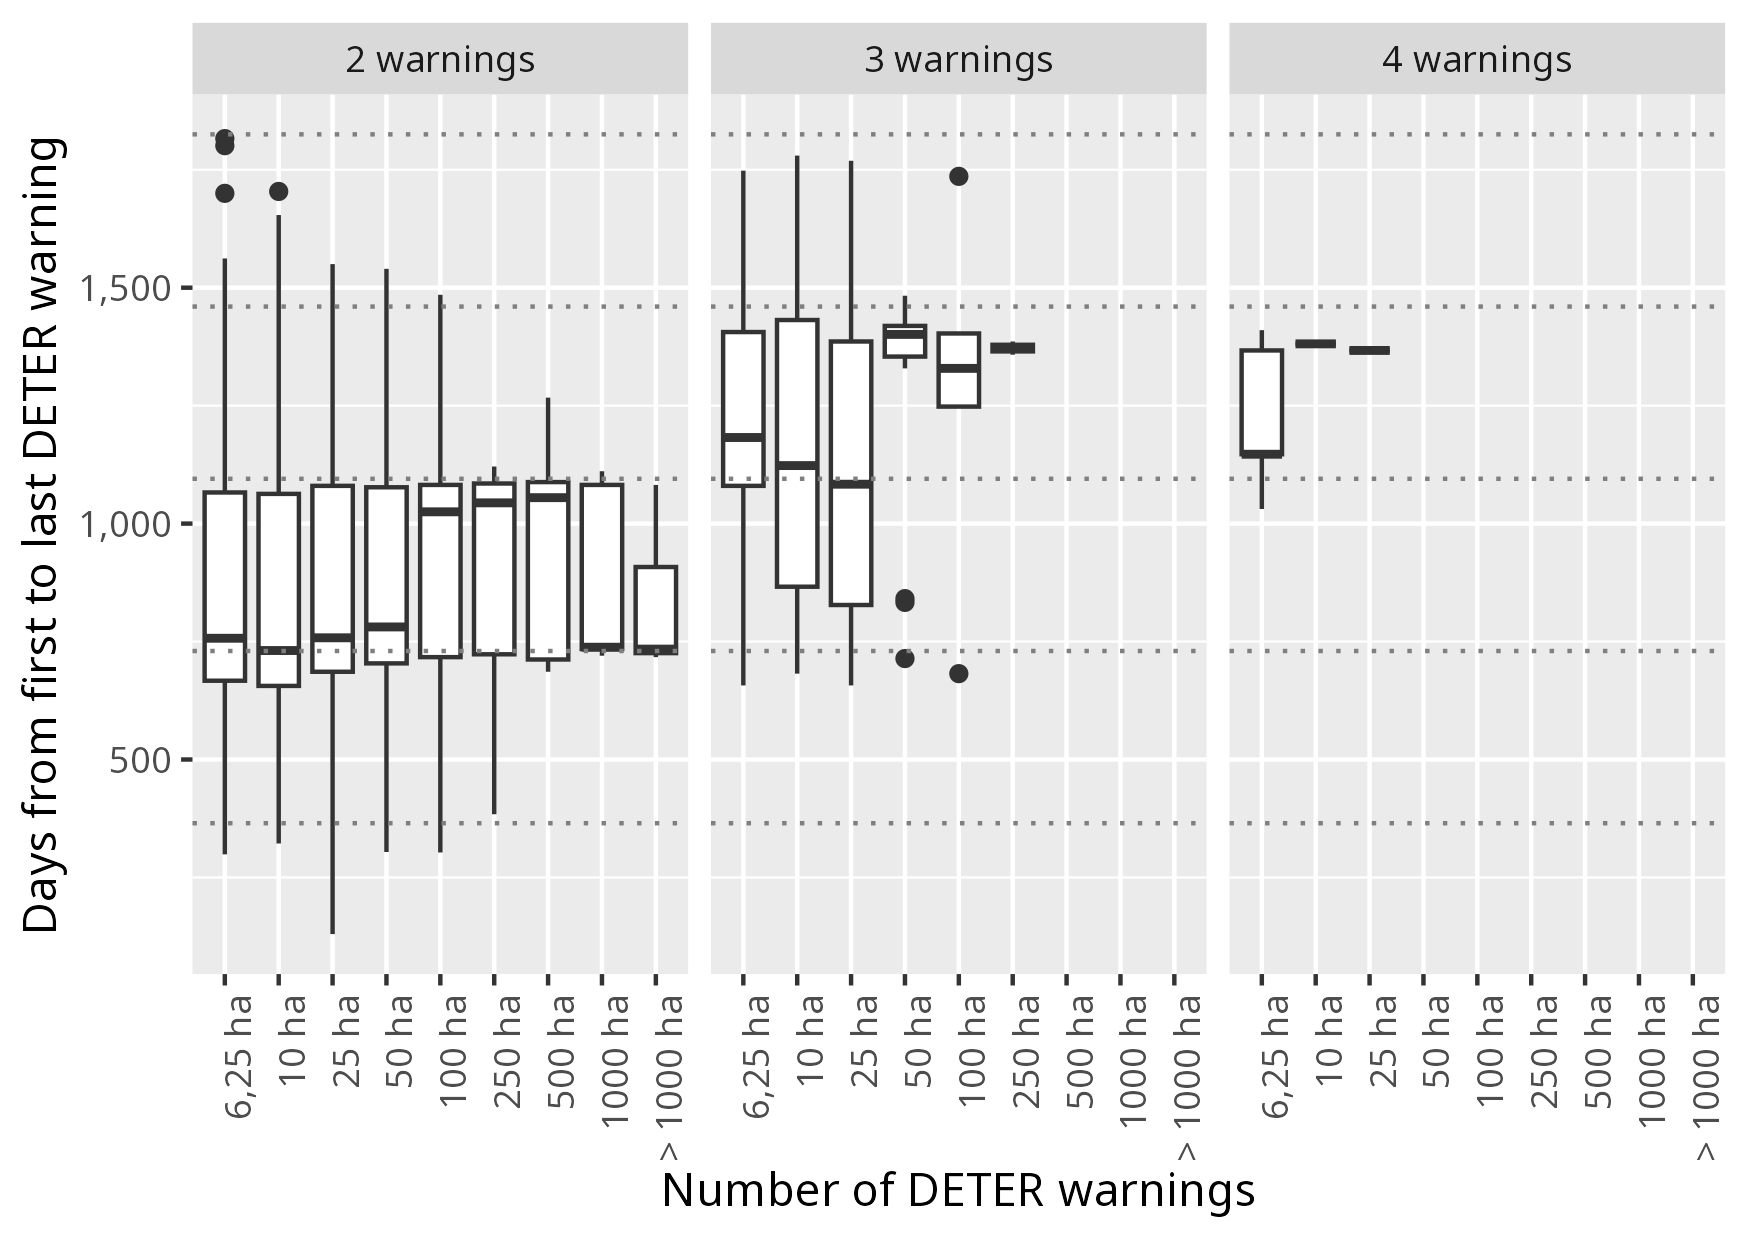
\includegraphics[width=\linewidth]{plot_days_first_to_last.png}
    \caption{Number of days between the first and last DETER warning of the 
        same subarea. Note how the difference between 2 and 3 warnings is 
        approximately 365 days (dotted lines). Each Box plot shows the median; 
        the first and third quartiles (hinges); 1.5 times the inter-quartile 
        range from the hinges; and the outliers.}
    \label{fig:plot_days_first_to_last}
    \end{center}
\end{figure}

